\documentclass[journal,12pt,twocolumn]{IEEEtran}
%
\usepackage{setspace}
\usepackage{gensymb}
%\doublespacing
\singlespacing

%\usepackage{graphicx}
%\usepackage{amssymb}
%\usepackage{relsize}
\usepackage[cmex10]{amsmath}
%\usepackage{amsthm}
%\interdisplaylinepenalty=2500
%\savesymbol{iint}
%\usepackage{txfonts}
%\restoresymbol{TXF}{iint}
%\usepackage{wasysym}
\usepackage{amsthm}
%\usepackage{iithtlc}
\usepackage{mathrsfs}
\usepackage{txfonts}
\usepackage{stfloats}
\usepackage{bm}
\usepackage{cite}
\usepackage{cases}
\usepackage{subfig}
%\usepackage{xtab}
\usepackage{longtable}
\usepackage{multirow}
%\usepackage{algorithm}
%\usepackage{algpseudocode}
\usepackage{enumitem}
\usepackage{mathtools}
\usepackage{tikz}
\usepackage[american]{circuitikz}
\usepackage{verbatim}
\usepackage{tfrupee}
\usepackage[breaklinks=true]{hyperref}
%\usepackage{stmaryrd}
\usepackage{tkz-euclide} % loads  TikZ and tkz-base
\usetkzobj{all}
\usetikzlibrary{decorations.markings}
\usetikzlibrary{shapes.geometric}
\newif\iflabrev
\usepackage{listings}
    \usepackage{color}                                            %%
    \usepackage{array}                                            %%
    \usepackage{longtable}                                        %%
    \usepackage{calc}                                             %%
    \usepackage{multirow}                                         %%
    \usepackage{hhline}                                           %%
    \usepackage{ifthen}                                           %%
  %optionally (for landscape tables embedded in another document): %%
    \usepackage{lscape}     
\usepackage{multicol}
\usepackage{chngcntr}
%\usepackage{enumerate}

%\usepackage{wasysym}
%\newcounter{MYtempeqncnt}
\DeclareMathOperator*{\Res}{Res}
%\renewcommand{\baselinestretch}{2}
\renewcommand\thesection{\arabic{section}}
\renewcommand\thesubsection{\thesection.\arabic{subsection}}
\renewcommand\thesubsubsection{\thesubsection.\arabic{subsubsection}}

\renewcommand\thesectiondis{\arabic{section}}
\renewcommand\thesubsectiondis{\thesectiondis.\arabic{subsection}}
\renewcommand\thesubsubsectiondis{\thesubsectiondis.\arabic{subsubsection}}

% correct bad hyphenation here
\hyphenation{op-tical net-works semi-conduc-tor}
\def\inputGnumericTable{}                                 %%

\lstset{
%language=C,
frame=single, 
breaklines=true,
columns=fullflexible
}
%\lstset{
%language=tex,
%frame=single, 
%breaklines=true
%}

\begin{document}
%


\newtheorem{theorem}{Theorem}[section]
\newtheorem{problem}{Problem}
\newtheorem{proposition}{Proposition}[section]
\newtheorem{lemma}{Lemma}[section]
\newtheorem{corollary}[theorem]{Corollary}
\newtheorem{example}{Example}[section]
\newtheorem{definition}[problem]{Definition}
%\newtheorem{thm}{Theorem}[section] 
%\newtheorem{defn}[thm]{Definition}
%\newtheorem{algorithm}{Algorithm}[section]
%\newtheorem{cor}{Corollary}
\newcommand{\BEQA}{\begin{eqnarray}}
\newcommand{\EEQA}{\end{eqnarray}}
\newcommand{\define}{\stackrel{\triangle}{=}}
\bibliographystyle{IEEEtran}
%\bibliographystyle{ieeetr}
\providecommand{\mbf}{\mathbf}
\providecommand{\pr}[1]{\ensuremath{\Pr\left(#1\right)}}
\providecommand{\qfunc}[1]{\ensuremath{Q\left(#1\right)}}
\providecommand{\sbrak}[1]{\ensuremath{{}\left[#1\right]}}
\providecommand{\lsbrak}[1]{\ensuremath{{}\left[#1\right.}}
\providecommand{\rsbrak}[1]{\ensuremath{{}\left.#1\right]}}
\providecommand{\brak}[1]{\ensuremath{\left(#1\right)}}
\providecommand{\lbrak}[1]{\ensuremath{\left(#1\right.}}
\providecommand{\rbrak}[1]{\ensuremath{\left.#1\right)}}
\providecommand{\cbrak}[1]{\ensuremath{\left\{#1\right\}}}
\providecommand{\lcbrak}[1]{\ensuremath{\left\{#1\right.}}
\providecommand{\rcbrak}[1]{\ensuremath{\left.#1\right\}}}
\theoremstyle{remark}
\newtheorem{rem}{Remark}
\newcommand{\sgn}{\mathop{\mathrm{sgn}}}
\providecommand{\abs}[1]{\left\vert#1\right\vert}
\providecommand{\res}[1]{\Res\displaylimits_{#1}} 
\providecommand{\norm}[1]{\left\lVert#1\right\rVert}
%\providecommand{\norm}[1]{\lVert#1\rVert}
\providecommand{\mtx}[1]{\mathbf{#1}}
\providecommand{\mean}[1]{E\left[ #1 \right]}
\providecommand{\fourier}{\overset{\mathcal{F}}{ \rightleftharpoons}}
%\providecommand{\hilbert}{\overset{\mathcal{H}}{ \rightleftharpoons}}
\providecommand{\system}{\overset{\mathcal{H}}{ \longleftrightarrow}}
	%\newcommand{\solution}[2]{\textbf{Solution:}{#1}}
\newcommand{\solution}{\noindent \textbf{Solution: }}
\newcommand{\cosec}{\,\text{cosec}\,}
\providecommand{\dec}[2]{\ensuremath{\overset{#1}{\underset{#2}{\gtrless}}}}
\newcommand{\myvec}[1]{\ensuremath{\begin{pmatrix}#1\end{pmatrix}}}
\newcommand{\mydet}[1]{\ensuremath{\begin{vmatrix}#1\end{vmatrix}}}
%\numberwithin{equation}{section}
\numberwithin{equation}{subsection}
%\numberwithin{problem}{section}
%\numberwithin{definition}{section}
\makeatletter
\@addtoreset{figure}{problem}
\makeatother
\let\StandardTheFigure\thefigure
\let\vec\mathbf
%\renewcommand{\thefigure}{\theproblem.\arabic{figure}}
\renewcommand{\thefigure}{\theproblem}
%\setlist[enumerate,1]{before=\renewcommand\theequation{\theenumi.\arabic{equation}}
%\counterwithin{equation}{enumi}
%\renewcommand{\theequation}{\arabic{subsection}.\arabic{equation}}
\def\putbox#1#2#3{\makebox[0in][l]{\makebox[#1][l]{}\raisebox{\baselineskip}[0in][0in]{\raisebox{#2}[0in][0in]{#3}}}}
     \def\rightbox#1{\makebox[0in][r]{#1}}
     \def\centbox#1{\makebox[0in]{#1}}
     \def\topbox#1{\raisebox{-\baselineskip}[0in][0in]{#1}}
     \def\midbox#1{\raisebox{-0.5\baselineskip}[0in][0in]{#1}}
\vspace{3cm}
\title{
%	\logo{
Trans-resistance Feedback Circuits
%	}
}
\author{V. L. Narasimha Reddy $^{*}$% <-this % stops a space
	\thanks{*The author is with the Department
		of Electrical Engineering, Indian Institute of Technology, Hyderabad
		502285 India. All content in this manual is released under GNU GPL.  Free and open source.}
	
}	
%\title{
%	\logo{Matrix Analysis through Octave}{\begin{center}\includegraphics[scale=.24]{tlc}\end{center}}{}{HAMDSP}
%}
% paper title
% can use linebreaks \\ within to get better formatting as desired
%\title{Matrix Analysis through Octave}
%
%
% author names and IEEE memberships
% note positions of commas and nonbreaking spaces ( ~ ) LaTeX will not break
% a structure at a ~ so this keeps an author's name from being broken across
% two lines.
% use \thanks{} to gain access to the first footnote area
% a separate \thanks must be used for each paragraph as LaTeX2e's \thanks
% was not built to handle multiple paragraphs
%
%\author{<-this % stops a space
%\thanks{}}
%}
% note the % following the last \IEEEmembership and also \thanks - 
% these prevent an unwanted space from occurring between the last author name
% and the end of the author line. i.e., if you had this:
% 
% \author{....lastname \thanks{...} \thanks{...} }
%                     ^------------^------------^----Do not want these spaces!
%
% a space would be appended to the last name and could cause every name on that
% line to be shifted left slightly. This is one of those "LaTeX things". For
% instance, "\textbf{A} \textbf{B}" will typeset as "A B" not "AB". To get
% "AB" then you have to do: "\textbf{A}\textbf{B}"
% \thanks is no different in this regard, so shield the last } of each \thanks
% that ends a line with a % and do not let a space in before the next \thanks.
% Spaces after \IEEEmembership other than the last one are OK (and needed) as
% you are supposed to have spaces between the names. For what it is worth,
% this is a minor point as most people would not even notice if the said evil
% space somehow managed to creep in.
% The paper headers
%\markboth{Journal of \LaTeX\ Class Files,~Vol.~6, No.~1, January~2007}%
%{Shell \MakeLowercase{\textit{et al.}}: Bare Demo of IEEEtran.cls for Journals}
% The only time the second header will appear is for the odd numbered pages
% after the title page when using the twoside option.
% 
% *** Note that you probably will NOT want to include the author's ***
% *** name in the headers of peer review papers.                   ***
% You can use \ifCLASSOPTIONpeerreview for conditional compilation here if
% you desire.
% If you want to put a publisher's ID mark on the page you can do it like
% this:
%\IEEEpubid{0000--0000/00\$00.00~\copyright~2007 IEEE}
% Remember, if you use this you must call \IEEEpubidadjcol in the second
% column for its text to clear the IEEEpubid mark.
% make the title area
\maketitle
%\newpage
%\tableofcontents
\bigskip
\renewcommand{\thefigure}{\theenumi}
\renewcommand{\thetable}{\theenumi}
%\renewcommand{\theequation}{\theenumi}
%\begin{abstract}
%%\boldmath
%In this letter, an algorithm for evaluating the exact analytical bit error rate  (BER)  for the piecewise linear (PL) combiner for  multiple relays is presented. Previous results were available only for upto three relays. The algorithm is unique in the sense that  the actual mathematical expressions, that are prohibitively large, need not be explicitly obtained. The diversity gain due to multiple relays is shown through plots of the analytical BER, well supported by simulations. 
%
%\end{abstract}
% IEEEtran.cls defaults to using nonbold math in the Abstract.
% This preserves the distinction between vectors and scalars. However,
% if the journal you are submitting to favors bold math in the abstract,
% then you can use LaTeX's standard command \boldmath at the very start
% of the abstract to achieve this. Many IEEE journals frown on math
% in the abstract anyway.
% Note that keywords are not normally used for peerreview papers.
%\begin{IEEEkeywords}
%Cooperative diversity, decode and forward, piecewise linear
%\end{IEEEkeywords}
% For peer review papers, you can put extra information on the cover
% page as needed:
% \ifCLASSOPTIONpeerreview
% \begin{center} \bfseries EDICS Category: 3-BBND \end{center}
% \fi
%
% For peerreview papers, this IEEEtran command inserts a page break and
% creates the second title. It will be ignored for other modes.
%\IEEEpeerreviewmaketitle
%\begin{abstract}
%The objective of this manual is to introduce control system design at an elementary level.
%\end{abstract}
%\section{Trans-resistance Feedback Circuits}
\begin{enumerate}[label=\thesubsection.\arabic*.,ref=\thesubsection.\theenumi]
\numberwithin{equation}{enumi}
\item A feedback control system has the characteristic equation 
\begin{align}
    s^2 + 6Ks + 2s + 5 = 0, \quad K > 0. 
\label{eq:ee18btech11046_char}
\end{align}
%
Find the open loop gain.
\\
\solution     \label{eq:ee18btech11046_char} can be expressed as

\begin{align}
    1+\frac{6 k s}{s^{2}+2 s+5}&=0    
\\
\implies 1+KG(s)&=0
\\
\implies G(s) &= \frac{6 s}{s^{2}+2 s+5}
\label{eq:ee18btech11046_gs}
\end{align}

\item Find the poles and zeros of $G(s)$
\\
\solution The poles and zeros  are at 
\begin{align}
\begin{split}
p_1,p_2 &= -1 \pm 2\j
\\
z &=0
\end{split}
\label{eq:ee18btech11046_pz}
\end{align}

\item Find the number of root locus branches.
\\
\solution  For $G(s)$, let 
\begin{itemize}
\item $P$- No. of finite poles
\item $Z$- No. of finite zeros
\end{itemize}
%
The number of root locus branches
\begin{align}
N = 
\begin{cases}
P & P > Z,
\\
Z & P < Z.
\end{cases}
\end{align}
The root locus branches start at the open loop poles and end at open loop zeros. 
From \eqref{eq:ee18btech11046_pz}, 
\begin{align}
P=2, Z = 1 \implies N = 2
\end{align}
%
One branch originates at each pole and ends at zero and the other branch starts from other pole and goes to infinity.
\item Find the centroid and the angle of asymptotes.
\\
\solution 
Some of the root locus branches approach infinity when $P \ne Z$. Asymptotes give the direction of these root locus branches. The intersection point of asymptotes on the real axis is known as centroid.  The ordinate of the centroid is given by 
\begin{align}
\frac{\sum_{i=1}^{P} p_{i}-\sum_{j=1}^{Z} z_{j}}{P-Z} 
&= \frac{-2-0}{2-1}
\\
&= -2
\end{align}
%
after substituting from \eqref{eq:ee18btech11046_pz}.  Thus, the centroid is at $\brak{-2,0}$.
The formula for angle of asymptotes $\theta$ is
\begin{align}
\theta&=\frac{(2 q+1) \pi}{P-Z}, \quad q =0, 1, \dots P-Z-1
\\
&=\pi
\end{align}
%
One branch meets the real axis at a breakaway point then goes to zero at origin and other goes to infinity following the asymptote($y=0$).
	\item Find the intersection points of root locus branches with the imaginary axis. 
\\
\solution Using the Routh array method, 

\item Find the angle of departure with respect to the  pole $p_k$.
\\
\solution The angle of departure with respect to the $k$th (complex) pole is defined as 
\begin{align}
\phi_{k}^{d}&=
\begin{cases}
\pi-\phi_k, &  \text{Im}\brak{p_k} \ne 0
\\
0 & \text{Im}\brak{p_k} = 0
\end{cases}
\end{align}
where,
\begin{align}
\phi_k&=\sum_{i=1}^{P} \phase{p_i-p_k}-\sum_{j}^{Z} \phase{p_k - z_{j}}
\end{align}
%
For $p_1 = -1+2\j$, 
\begin{align}
\phi_{1} &= \phase{-1+2\j-\brak{-1-2\j}} - \phase{-1+2i-0}
\\
\implies  &= \frac{\pi}{2} + \brak{\pi - \tan^{-1}2} = \frac{3\pi}{2} - \tan^{-1}2
\end{align}
%
\item Find the angle of arrival with respect to the zero $z_k$
\\
\solution The angle of arrival with respect to the $k$th (complex) zero is defined as 
\begin{align}
\phi_{k}^{a}&=
\begin{cases}
\pi-\phi_k, &  \text{Im}\brak{z_k} \ne 0
\\
0 & \text{Im}\brak{z_k} = 0
\end{cases}
\end{align}
where,
\begin{align}
\phi_k&=\sum_{i=1}^{P} \phase{z_k-p_i}-\sum_{j}^{Z} \phase{z_k - z_{j}}
\end{align}
%
Since there are no complex zeros there is no angle of arrival.

\item Find the breakaway point for the root locus.
\\
\solution From \eqref{eq:ee18btech11046_char} and 
\eqref{eq:ee18btech11046_gs},
    \begin{align}
        K&=\frac{-\left(s^{2}+2 s+5\right)}{6 s},
\\
        \frac{d K}{d s}&=0 \implies \sbrak{1-\frac{5}{s^{2}}}=0 
\\
  \implies        s&=-\sqrt{5}
    \end{align}
%
which is the  breakaway point that lies only in the left half plane. Some information on the breakaway point is available below.
\begin{itemize}
\item While varying $K$, the point where the Root Locus enters the real axis is called th breakaway point.
\item   It is the point on a real axis segment of the root locus between two real poles where the two real closed-loop poles meet and diverge to become complex conjugates.
\item  As the root locus is symmetric about the real axis there will be two roots at the breakaway point. 

\end{itemize}
    
\item Plot the Root Locus.
\\
\solution The following code generates the desired plot in Fig. \ref{fig:ee18btech11046}.
\begin{lstlisting}
codes/ee18btech11046.py
\end{lstlisting}    


\begin{figure}[ht!]
\centering
    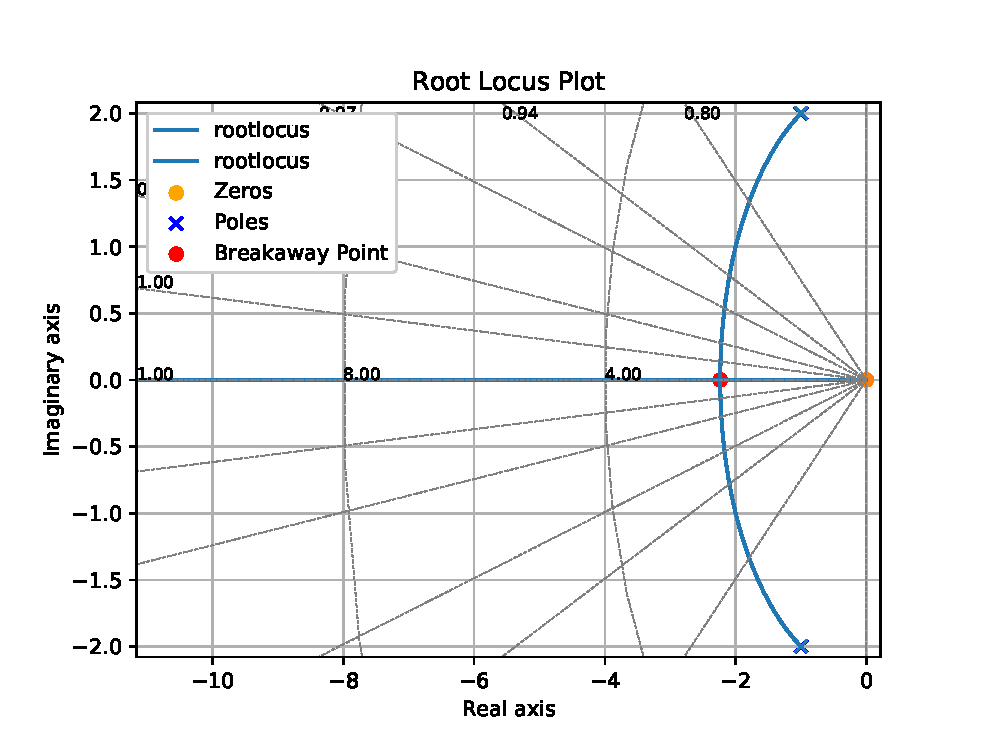
\includegraphics[width=\columnwidth]{./figs/ee18btech11046.eps}
    \caption{}
    \label{fig:ee18btech11046}
\end{figure}


\end{enumerate}


\end{document}
